\newacronym{LDA}{LDA}{Latent Dirichlet Allocation}
\newacronym{nltk}{NLTK}{Natural Language Toolkit}
\section{Classification}
\label{sec:classification}
\subsection{Overview}
Classification is currently an
very active area of research \autocite{Zhang2000}, especially with respect to
internet documents. Classification is a branch of machine learning which
attempts to predict the underlying topic, or classification of a given document.
As a discipline under machine learning it's helpful to describe machine learning
at a high level, before describing the classification techniques evaluated and
finally implemented in CloudAssure
%TODO Add the classifiction overview diagram to this section

\subsection{Machine Learning with Respect to Classification}
Machine Learning can be described as a mathematical model which reverses a human
process \autocite{Bishop2009}. In the area of classification this is
a straightforward description. For example, a given document is composed of words which
intend to persuade or inform the reader (See
Figure~\ref{fig:LDA_Generative_Model}) Thus, the documents words are related
by some list of topics \autocite{Blei2009}. Topic Models supposes that documents are
written in the following fashion:
\begin{enumerate}
    \item The author has a finite set of lists. Each list contains a vocabulary
        for a given topic.
    \item The author chooses to start writing a document.
    \item The author rolls a die to choose a topic list.
    \item The author rolls the die again to choose a word from the selected
        topic list.
    \item The author writes down the word.
    \item The author continues rolling the die until the document is of sufficient
        length.
    \item Once the document is complete, the author destroys the topic lists.
\end{enumerate}

\begin{figure}[h!]
    \begin{center}
        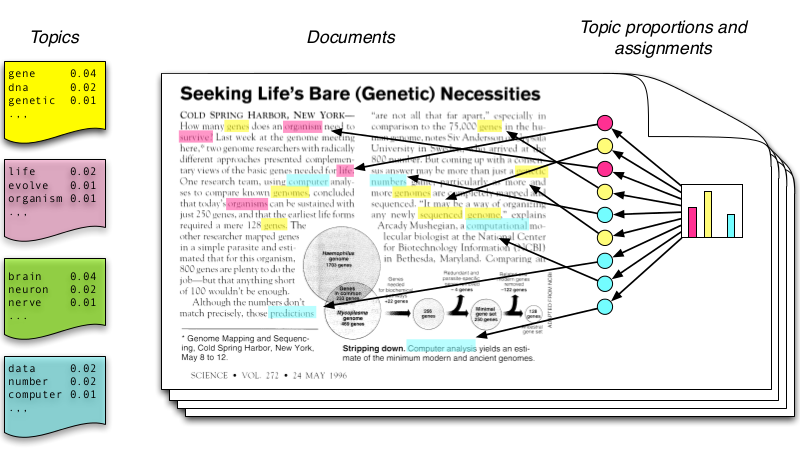
\includegraphics[width=0.90\textwidth]{Figures/LDA_Generation.png}
        \caption{Example of the LDA Generative Document Model}
        \label{fig:LDA_Generative_Model}
    \end{center}
\end{figure}
Now given any document, what are the topics contained in it? The original topic
lists were destroyed, so Topic Models proposes a method to recreate them. Thus reversing
the process of writing a document.

Topic Models is only one example, but all classification methods use some algorithm which assumes a specific
distribution to the document with the intent of extracting some unobservable
property. During the course of designing CloudAssure's classification module, we looked at a number of techniques
including Topic Models, Neural Nets, Bayesian Inference, and finally, Decision Trees.

\subsubsection{Probabilistic Topic Models}
In ``Probabilistic Topic Models'', Blei describes the Latent Dirichlet
Allocation and its probabilistic approach to topic prediction
\autocite{Blei2012}. Topic Models is different among the classical classifiers we
surveyed for CloudAssure. As described above, Topic Models supposes documents are
distributed according to the \gls{LDA}. Blei then uses this generative model to 
show how the original topic lists can be
recomposed from the document. This technique is very powerful for discovering
topics in a document, but for our usecase, there is a second step of
grouping those newly discovered topics into classifications
\autocite{RadimRehurek2010}. Due to this secondary step, we
choose not to use the Topic Model algorithm.

\subsubsection{Neural Nets}
Neural Nets are another powerful classification technique. An artificial neural
net's power
extends from its non-linearity \autocite{Zhang2000}. A neural net is composed of
a number of nodes connected by a ``hidden'' layer. The input nodes
then filter features through this hidden layer which triggers select outputs
thus classifying a document \autocite{Merkl}. The neural net is very good at
doing this. However the ``hidden layer'' is, by definition, unobservable, and
the results are not readily traceable (i.e. given a result one cannot easily trace to
find the series of decision which lead to that decision). This increases the
complexity of implementation and debugging. Secondly, neural nets are sensitive
to their input data, more so that other techniques, thus a great deal of time
needs to be spent the to tune input features. For these two reasons, we choose not
to implements the Neural Net technique for CloudAssure's classification model.

\subsubsection{Bayesian Inference}
Bayesian Inference is a classical technique leveraging Bayes Theorem of
conditional probabilities as stated in equation \ref{eq:BayesTheorum}.
\begin{equation}
    P(A|B) = \frac{P(B | A) P(A)}{P(B)}
    \label{eq:BayesTheorum}
\end{equation}

In Equation \ref{eq:BayesTheorum} we see how to reverse the condition on
a conditional probability.  This reversal is precisely the goal of
classification in general \autocite{Bishop2009}. Bayesian classifiers are used
extensively in spam filters. Equation~\ref{eq:BayesSpam} states the
question, what is the probability a document is spam, given it contains the word
``Prescription''? 

\begin{equation}
    P(\text{spam} | \text{Prescription}) = \frac{P(\text{Prescription}
    | \text{spam}) \cdot P(\text{spam})}{P(\text{Prescription})}
    \label{eq:BayesSpam}
\end{equation}

From this, we see how we can classify a document given a single word, but
document are actually more complex than this.
Equation~\ref{eq:BayesSpamMedicine} asks the question more elegantly: What is
the probability a document is spam given it contains \emph{both} Prescription, and
medicine. 

\begin{equation}
    P(\text{spam} | \text{Prescription}, \text{medicine})
    = \frac{P(\text{Prescription}
    | \text{spam} \cap \text{medicine} ) \cdot P(\text{medicine}
    | \text{spam}) \cdot P(\text{spam})}{P(\text{Prescription})}
    \label{eq:BayesSpamMedicine}
\end{equation}

The Na\"{\i}ve Bayesian allows us to aggregate as many terms as we need to classify
a document. As we'll see in the implementation, CloudAssure uses the probability of 5,000
separate words to classify documents. Out of this analysis,  Bayesian
Inference is
suitable for CloudAssure, but we continued looking for a methodology that could
give better accuracy.
\subsubsection{Decision Trees}
The final technique we surveyed for a classification technique is the Decision
Tree. The Decision Tree divides the search space into a tree. This tree can be
described as a series of nested if statements as in
Algorithm \ref{alg:decision_tree}. Each branch of the
tree prunes a set of features from the search space reducing the features to
check at each decision \autocite{Segaran2008}. This tree structure is
proportional to the size of the training set, and our experiments show it to be
only 15\% smaller than the training set, while the frequency distribution table
for the Bayesian implementation is 84\% smaller than the training set. Despite
the increased memory load for this technique, we found the classification
results to be more accurate than the Bayesian method, and included it in
CloudAssure.

\begin{algorithm}
    \caption{Example how the decision tree can be divided into a series of
    nested if statements}
    \label{alg:decision_tree}
\begin{algorithmic}
    \If{ contains(professor) == False}
        \If{ contains(course) == False}
            \If{ contains(syllabus) == False}
                \If{ contains(faculty) == False} 
                    \Return{ u'Student'}
                \EndIf
                 \If{ contains(faculty) == True} 
                    \Return{ u'Student'}
                \EndIf
                \If{ contains(syllabus) == True}
                        \If{ contains(faculty) == False} 
                            \Return{ u'Course'}
                        \EndIf
                        \If{ contains(faculty) == True} 
                            \Return{ u'Faculty'}
                        \EndIf
                        \If{ contains(course) == True}
                            \If{ contains(interests) == False}
                                \If{ contains(resume) == False} 
                                        \Return{ u'Course'}
                                \EndIf
                            \EndIf
                        \EndIf
                    \EndIf
                \EndIf
            \EndIf
        \EndIf
\end{algorithmic}
\end{algorithm}

\subsection{Implementation}
The Classification System
needs to be properly trained for the best performance \autocite{Russell2008}.
CloudAssure has two provided algorithms: Bayesian and Decision Tree.
Depending on the implementor's dataset, one will offer more accurate results.

To be useful, the Classifier should provide a statically significant improvement over simply
guessing a category. For instance, if the dataset contains 4 categories, then
random chance will classify a document in the correct category 25\% of the time.
CloudAssure's classifier must do more accurate job than this.
Table~\ref{tab:classification_accuracy} summarizes the results for the example
dataset \autocite{University}.
\FloatBarrier 
\begin{table}[h!]
    \centering
    \begin{tabular}{c | c }
        \hline
        Classification Method & Accuracy \\
        \hline \hline
        Random Chance & 25\%\\
        Bayesian & 82.54\% \\
        Decision Tree & 86.87\% \\
    \end{tabular}
    \caption{Summary Accuracies of varying classification methods.}
    \label{tab:classification_accuracy}
\end{table}
\FloatBarrier
Our implementation is divided into two phases: A Direct Implementation, and
a second implementation utilizing the \gls{nltk}. \gls{nltk} provides a set of
tools and libraries accelerated by the SciPy and NumPy numerical libraries.
These libraries are hand-tuned FORTRAN implementations of advanced numerical
techniques. These techniques help alleviate the quirkiness of floating point.
Furthermore, \gls{nltk} defines tokenizers and other useful tools for
implementing natural language processing algorithms. The initial implementation was
a direct application of Bayes theorem in Python. This implementation resulted in
several faults however. Performance was poor, and classifying a large number of
documents resulted in floating point underflows, and other implementation
specific faults. There exists techniques to repair these problems such as
rewriting a products  of terms as a sum of \(log(terms) \) \autocite{Graham-Cummings2005}. \gls{nltk} however
already implements these techniques in a fast and correct manner. Thus, our results
are based on phase two, which uses \gls{nltk} as a math backend.\autocite{Denoyer2004}

\subsection{Training the Classifiers}
Instantiating the Classifier component of CloudAssure in one's facility is broken
into 4 steps:
\begin{enumerate}
    \item Choose a Dataset
    \item Define Feature Extraction.
    \item Train the 2 provided classifiers to determine which method best
        fits your configuration
    \item Save the plk file for future classifications
\end{enumerate}

\subsubsection{Choosing a DataSet}
The dataset must be categorized into the classifications ones company needs to
utilize. It seems pedantic, but the classifiers chosen for CloudAssure cull
new classifications from the data. The classifiers can only categorize data into
given categories. It is critically important that the dataset is evenly distributed across the
categories, and that the definition of each category is not ambiguous. 
Once a dataset is chosen one may begin feature selection.

\subsubsection{Extracting Features}
Feature selection is important to disambiguate the categories, especially for
more sensitive classifiers such as the Neural Net. The stock feature
selection in CloudAssure uses an industry standard list of stop words to remove
overly common or overly rare words from the features extracted from documents.
Once these words are pruned, it chooses the top 5,000 features. These parameters are tunable
 to get the best results.

\subsubsection{Creating a Database}
Once features have been selected, one may use the python examples to create
a training database. This is done with the following command: 
\texttt{python main.py --learn categoryFolders --name CategoryName}. Python
will recursively search the categoryFolders, extract all features and load
them into a database. Run this step multiple times for as many folders of
training data exist. This step outputs a database file used for training the
classifiers.

\subsubsection{Creating a plk file}
Once the database has been built, one may build the persistent classifier,
stored as a Python Pickle. Python Pickle is a binary format in the standard
Python library which allows one to persist any class instance to disk. This
allows CloudAssure to
be reloaded a trained classifier on demand. The following command will load all features from the
database and create a Bayesian model and save it as Bayesian-model.plk: 
\texttt{python main.py --type Bayes --model Bayesian-model.pkl}
Do this also for the decision tree: \texttt{python main.py --type Tree --model
decision-model.pkl}. Each training step will print out the accuracy, and the top
most influential features. This data can be used to tune the classifiers to an organization's needs.
This is by far the most time intensive step of the process. For our example dataset the tree
model for 3,695 documents took 75 minutes (86.87\% accurate) and the Bayes
model for 3,695 documents took 3 minutes (82.54\% accurate) as summarized by
Table~\ref{tab:classification_accuracy}. This took several
tuning iterations before accuracy levels were sufficient.

Once the classifier is sufficiently accurate one may use this model to classify
any document: \texttt{python main.py --classify document.html --name Bayesian-model.pkl}

 

\subsubsection{Security Concerns}
It is critically important that the .plk file be stored in a secure place, or be
cryptographically secured and verified prior to each load. The .plk file, if
manipulated by a maleficent agent, can be used to subvert the trust system and
classify data into any a document to the category of the agent's choosing.  


